The state pattern is a behavioral software design pattern. An object changes its class when its internal state changes. To illustrate the idea imagine that our vending machine \textit{VM} is a mobile vending machine and that it is connected by a wireless link $talk$ to a shop \textit{Shop1}. On signal fading \textit{Shop1} decides to send the link \textit{talk} to another shop \textit{Shop2} through the link \textit{switch} as shown in \refFig{fig_oz_mobile_vending_machine_and_shops}. \oz{} can be used to model the shop with considering the state pattern. When \textit{switch} occurs
\begin{itemize}
\item \textit{Shop1} sends \textit{talk} via \textit{switch} and changes its class from \textit{ActiveShop} to \textit{IdleShop} as shown in \refFig{fig_oz_active_idle_shop}.
\item \textit{Shop2} receives \textit{talk} via  \textit{switch} and changes its class from \textit{IdleShop} to \textit{ActiveShop} as shown in \refFig{fig_oz_active_idle_shop}.
\end{itemize}
Notice, when an object changes its class it keeps its state variables and skips the \textit{Init} schema of the new class.
\begin{figure}[H]%
\centering
\subcaptionbox{Before switch}{\fbox{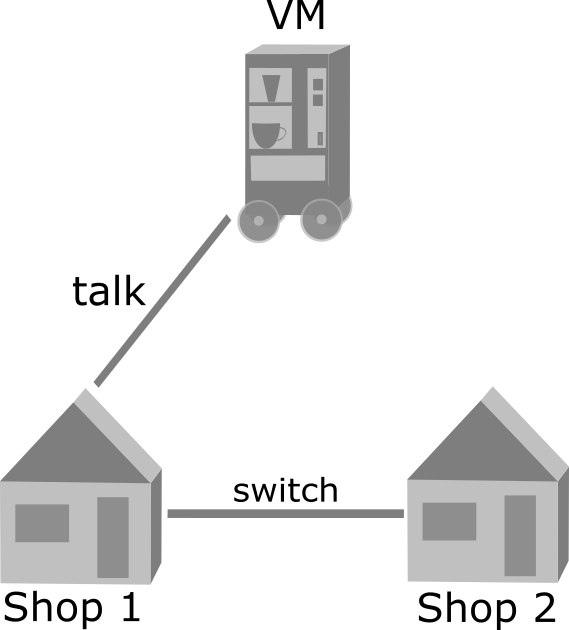
\includegraphics[width=0.45\textwidth]{./images/preliminaries/oz/oz_mobile_vending_machine_and_shops1.png}}}%
\hfill
\subcaptionbox{After switch}{\fbox{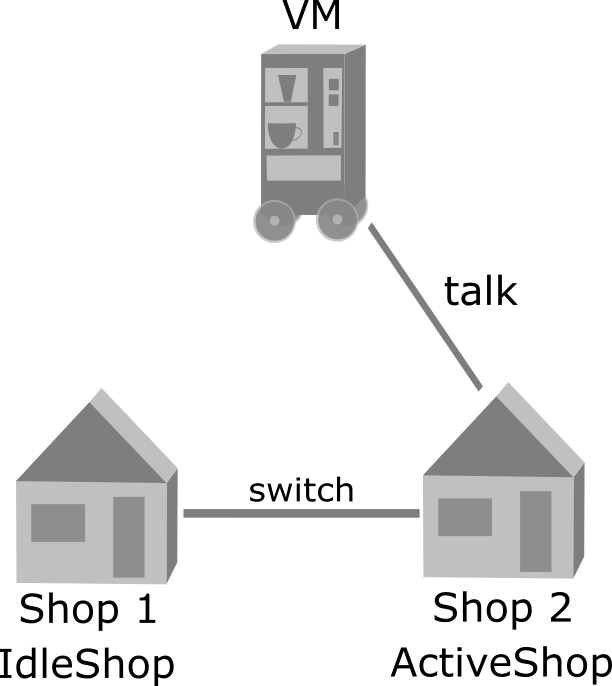
\includegraphics[width=0.45\textwidth]{./images/preliminaries/oz/oz_mobile_vending_machine_and_shops2.png}}}%
\caption{Mobile vending machine and shops}
\label{fig_oz_mobile_vending_machine_and_shops}%
\end{figure}

\begin{figure}[H]
\centering
\begin{sidebyside}
\begin{class}{ActiveShop(id: \integer)}
\\
\begin{state}
self, vmId, message: \integer
\\transferableOperation: nil | talk
\end{state} 
\\
\begin{init}
\\self = id
\\transferableOperation = talk
\end{init} 
\\
\begin{op}{switch\_\_\_\_\ then\ IdleShop}
x!: nil | talk
\ST
x! = transferableOperation
\\transferableOperation' = nil
\end{op}
\\
\begin{op}{talk}
\Delta (vmId, message)
\\y?, z?: \integer
\ST
y? = message'
\\z? = vmId'
\end{op}
\end{class}
\nextside
\begin{class}{IdleShop(id: \integer)}
\\
\begin{state}
self, vmId, message: \integer
\\transferableOperation: nil | talk
\end{state} 
\\
\begin{init}
\\self = id
\\transferableOperation = nil
\end{init} 
\\
\begin{op}{switch\_\_\_\_\ then\ ActiveShop}
\Delta (transferableOperation)
\\x?: nil | talk
\ST
x? = transferableOperation'
\end{op}
\end{class}
\end{sidebyside}
\caption{Active and idle shop.}
\label{fig_oz_active_idle_shop}
\end{figure}

